
\documentclass[11pt]{article}

% math packages
\usepackage{mathtools}
\usepackage{amsmath}
\usepackage{amssymb}    % Math symbols such as \mathbb
\usepackage{amsthm}
\usepackage{pgfplots}   % plots
\usepackage[linesnumbered, boxruled,titlenumbered, noend]{algorithm2e} % algorithmn
% https://en.wikibooks.org/wiki/LaTeX/Algorithms
% http://ctan.mirror.rafal.ca/macros/latex/contrib/algorithm2e/doc/algorithm2e.pdf
\usepackage{listings} % code formatting
\usepackage{color}
\usepackage{tikz}
\usetikzlibrary{automata,positioning}


\definecolor{codegreen}{rgb}{0,0.6,0}
\definecolor{codegray}{rgb}{0.5,0.5,0.5}
\definecolor{codepurple}{rgb}{0.58,0,0.82}
\definecolor{backcolour}{rgb}{0.95,0.95,0.92}


\lstdefinestyle{mystyle}{
    backgroundcolor=\color{backcolour},
    commentstyle=\color{codegreen},
    keywordstyle=\color{magenta},
    numberstyle=\tiny\color{codegray},
    stringstyle=\color{codepurple},
    basicstyle=\footnotesize,
    breakatwhitespace=false,
    breaklines=true,
    captionpos=b,
    keepspaces=true,
    numbers=left,
    numbersep=5pt,
    showspaces=false,
    showstringspaces=false,
    showtabs=false,
    tabsize=2
}
\lstset{style=mystyle}




\SetKwProg{Fn}{Function}{}{}

% other packages
\usepackage{graphicx}
\graphicspath{ {../assets/} }
\usepackage{enumitem}
\usepackage[a4paper, total={6in, 8in}]{geometry}
\usepackage{hyperref}

% proper inline math display, adjust height for symbols like \sum
\everymath{\displaystyle}

% define tags for math use..
\theoremstyle{plain}% default
\newtheorem{theorem}{Theorem}[section]
\newtheorem{corollary}{Corollary}[theorem]

\theoremstyle{definition}
\newtheorem{defn}{Definition}
\newtheorem{exmp}{Example}[defn]
\newtheorem{prop}{Proposition}[defn]
\newtheorem{lemma}{Lemma}[defn]



\theoremstyle{remark}
\newtheorem*{rem}{Remark}
\newtheorem*{note}{Note}
\newtheorem{case}{Case}

% Gives begin{solution} same formating as \begin{proof}
\newenvironment{solution}
  {\begin{proof}[Solution]}
  {\end{proof}}


\newenvironment{approach}
  {\begin{proof}[Approach]}
  {\end{proof}}


%running fraction with slash - requires math mode.
\newcommand*\rfrac[2]{{}^{#1}\!/_{#2}}
%shortcut to mathbb
\newcommand{\N}{\mathbb{N}}
\newcommand{\R}{\mathbb{R}}
\newcommand{\I}{\mathbb{I}}
% color highlighting
\newcommand{\hilight}[1]{\colorbox{yellow}{#1}}

\title{CSC236 Assignment \#3}
\author{Zhongtian Ouyang, Peiqi Wang}

\begin{document}
\maketitle




\section*{Problem 1}

Proof of Correctness for iterative algorithms.
\begin{enumerate}
\item Design an iterative closest pair algorithm for finding the closest pair of points in 2D.\\
\emph{Precondition:} Input is a list of $n$ points in the form $(x_i,y_i)$, where $x_i,y_i\in\mathbb{R}$\\
\emph{Postcondition:} Return a closest pair of points


\begin{lstlisting}[language=Python]
  def closestPair(L):
      """ Brute force method for finding the closest pair of points from an array L of bivariate points (x_i, y_i)

      @param: Array[Array] L: input array
      @rparam: Array t: the closest pair
      """

      n = len(L)
      u, v = -1, -1
      min = float('inf')

      for i in range(0, n):
          for j in range(i+1, n):
              distance = findDistance(L[i], L[j])
              if distance < min:
                  min = distance
                  u = i
                  v = j
      return (L[u], L[v])

  def findDistance(p1, p2):
      return float(math.sqrt( (p1[0]-p2[0])**2 + (p1[1] - p2[1])**2 ))
\end{lstlisting}


\item Find complexity class
\begin{solution}
  $ $\\
  We notice that there is a nested loop consisting of an outer $i$ loop and inner $j$ loop. The outer $i$ loop executes $n-1$ times and the inner $j$ loop executes $n-i-1$ times. Therefore the nested loop executes
  \[
    (n-1) + (n-2) + \dots + 1 = \frac{n(n-1)}{2} = \frac{1}{2}n^2 - \frac{1}{2}n
  \]
  iterations. The complexity of class is therefore $\Theta{(n^2)}$

\end{solution}
\item Prove correctness:
  \begin{enumerate}
    \item Define Loop Invariant

    \begin{solution}
      $ $\\
      The loop invariant for the outer $i$ loop is

      \begin{center}
        $P(k):$ if outer loop is executed at least $k$ times, then $min$ contains the minimum distance between any point in $L[0..k-1]$ and any point in $L[0..n-1]$. And the indices of the corresponding closest points in $L$ are $u$ and $v$ respectively.
      \end{center}

      Here we use induction to prove that $P(i)$ holds for all $i\in \N$


       \textbf{Basis:} \\
       When $i=0$, $min$ is infinity and $u,v = -1$, Since there is no points at indices -1, $P(0)$ is true trivially. \\
       \textbf{Inductive step:} \\
       Let $i>0$. Assume $P(i)$ holds and we prove $P(i+1)$ holds as well.

       Here we use $P(i)$ as the precondition for the inner $j$ loop. Specifically, $min$ contains the minimum distance between any points in $L[0..i-1]$ and any point in $L[0..n-1]$ And the indices of the corresponding closest points in $L$ are $u$ and $v$ respectively. We define the loop invariant for the inner loop as follows,

       \begin{center}
         Q(k): if the inner loop is executed at least $k$ times, then $min$ is the minimum of \textbf{1)} minimum distance between any point in $L[0..i-1]$ and any point in $L[0..n-1]$. \textbf{2)} the minimum of $L[i]$ and any points in $L[i+1..i+1+k]$. Also the indices of the corresponding closest points in $L$ are $u$ and $v$ respectively.
       \end{center}

       We prove inner state invariant $Q(m)$ holds for all $m\in \N$, where $m$ denotes the iterations of inner loop traversed.

       \textbf{\textit{Basis: }}\\
       when $m=0$, before the inner loop first executes, precondition $P(i)$ holds, therefore $Q(0)$ holds.\\
       \textbf{\textit{Inductive step:}}\\
       when $m>0$, let $m$ be an arbitrary number such that $Q(m)$ holds, now we prove $Q(m+1)$ holds as well.
       \textit{case 1:} when $distance \geq min$, then $min$ remains to be the minimum given by $P(i)$ and $Q(m)$, therefore $Q(m+1)$ holds. \\
       \textit{case 1:} when $distance < min$. Notice in line 14 $distance$ denotes the distance beween $L[i]$ and $L[i+1+m+1]$, $min$ is assigned value of $distance$. Now $min$ is the minimum of
       \begin{enumerate}
         \item minimum between any points in $L[0..i-1]$ and any point in $L[0..n-1]$
         \item minimum betwen $L[i]$ and any points in $L[i+1..i+1+m]$
         \item minimum of $L[i]$ and $L[i+1..i+1+m+1]$
       \end{enumerate}
       $u$ and $v$ correspondingly assigned the indices of closest points. Therefore $Q(m+1)$ holds.

       Hence loop invariant $Q(m)$ holds for all $m\in\N$

       Therefore, if the inner loop terminates with $m = n-1$, then $min$ contains minimum of
       \begin{enumerate}
         \item the minimum distance between any points in $L[0..i-1]$ and any point in $L[0..n-1]$
         \item the minimum distance between $L[i]$ and any points in $L[0..n-1$]
       \end{enumerate}
       Therefore $min$ contains minimum of any points in $L[0..i]$ and any points in $L[0..n-1]$. Also by state invariant $Q$, $u,v$ are corresponding closest points. Therefore $P(i+1)$ holds.

       To conclude, by simple induction, we proved that state invariant $P(i)$ holds for all $i\in\N$

    \end{solution}
    \item Prove Partial Correctness
    \begin{solution}
      Prove,

      \begin{center}
        Suppose that the program executes and satisfies precondition. If the program terminates, when it does, the post condition holds.
      \end{center}

      When the outer for loop terminates, then $i=n-1$, by state invariant proved previously, $min$ is the minimum of any points in $L[0..n-2]$ and $L[0..n-1]$ and $u,v$ are corresponding indices of closest pair of points. We can see that this covers the entirety of points in the list. Therefore the returned pair of points $L[u], L[v]$ are pairs of points with minimum distance.

    \end{solution}
    \item Termination (use either theorem 2.5 in the notes or POW)
    \begin{solution}
      $ $\\
      For the inner loop,let $f_i=n-j_i$ for arbitrary iteration $i$, therefore $f_i$ is an integer because $n$ and $j_i$ are integers. Since $j_{i+1} = j_i + 1$ as a result of the for loop and $n$ is a finite integer, then $f_{i+1} < f_i$ for all $i$. $f_i$ are decreasing series of integers, hence there are only finitely many $f_i$. The inner loop therefore will terminate. \\

      For the outer loop. Let $g_l = n-i_l$ for arbitrary iteration $l$, therefore $g_l$ is an integer because $n$ and $i_l$ are integers. Since $i_{l+1}  = i_l + 1$ as a result of the for loop and $n$ is a finite integer, then $g_{l+1}<g_l$ for all $l$. $g_l$ is decreasing series of integers, hence there are finitely many $g_i$. Also for any iteration, the inner for loop will terminate, therefore the outer loop will terminate \\

      Hence the program terminates.
    \end{solution}
  \end{enumerate}
\end{enumerate}





\section*{Problem 2}
DFSAs and their operations
\begin{enumerate}
\item Define and draw DFSAs on binary alphabet $\Sigma=\{0,1\}$ for 2 languages: $L_1(M_1)$ = \{all strings with even number of characters in a string\}, $L_2(M_2)$ = \{all strings that have even number of $1$s\}

\begin{solution}
  $ $\\
  For $M_1$
  \begin{center}
    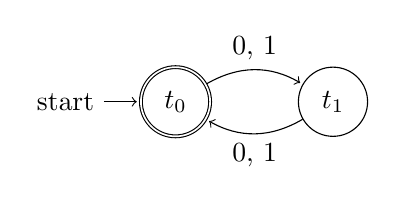
\begin{tikzpicture}[shorten >=1pt,node distance=2cm,on grid,auto]
     \node[state,initial, accepting] (t_0)   {$t_0$};
     \node[state] (t_1) [right=of t_0] {$t_1$};
      \path[->]
      (t_0) edge [bend left] node {0, 1} (t_1)
      (t_1) edge [bend left] node {0, 1} (t_0);
    \end{tikzpicture}
  \end{center}
  \begin{align*}
    Q &= \{t_0, t_1\}\\
    \Sigma &= \{0, 1\}\\
    s &= t_0 \\
    F &= \{t_0\} \\
    \delta &= Q \times \Sigma\text{ specified below}
  \end{align*}
  \begin{center}
    \begin{tabular}{|c | c c|}
    \hline
     & 0 & 1 \\
    \hline
    $t_0$ & $t_1$ & $t_1$ \\
    \hline
    $t_1$ & $t_0$ & $t_0$ \\
    \hline
   \end{tabular}
  \end{center}

  For $M_2$
  \begin{center}
    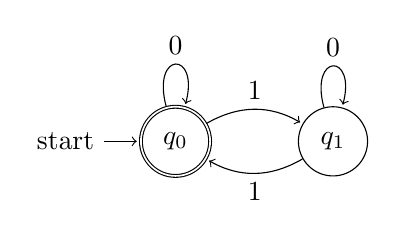
\begin{tikzpicture}[shorten >=1pt,node distance=2cm,on grid,auto]
     \node[state,initial, accepting] (q_0)   {$q_0$};
     \node[state] (q_1) [right=of q_0] {$q_1$};
      \path[->]
      (q_0) edge [bend left]  node {1} (q_1)
            edge [loop above] node {0} ()
      (q_1) edge [bend left]  node {1} (q_0)
            edge [loop above] node {0} ();
    \end{tikzpicture}
  \end{center}
  \begin{align*}
    Q &= \{q_0, q_1\}\\
    \Sigma &= \{0, 1\}\\
    s &= q_0 \\
    F &= \{q_0\} \\
    \delta &= Q \times \Sigma\text{ specified below}
  \end{align*}
  \begin{center}
    \begin{tabular}{|c | c c|}
    \hline
     & 0 & 1 \\
    \hline
    $q_0$ & $q_0$ & $q_1$ \\
    \hline
    $q_1$ & $q_1$ & $q_0$ \\
    \hline
   \end{tabular}
  \end{center}
\end{solution}

\item Identify DFSA $M_3$ for the union of languages $L_1\cup L_2$ - you can define it formally (don't need to draw).

\begin{solution}
  $ $\\
  We can construct DFSA $M_3$ for $L_1\cup L_2$ by,
  \begin{align*}
    Q &= \{(t_0, q_0), (t_0, q_1), (t_1, q_0), (t_1, q_1)\}\\
    \Sigma &= \{0, 1\}\\
    s &= (t_0, q_0) \\
    F &= \{(t_0, q_0), (t_0, q_1), (t_1, q_0)\} \\
    \delta &= Q \times \Sigma\text{ specified below}
  \end{align*}
  \begin{center}
    \begin{tabular}{|c | c c|}
    \hline
     & 0 & 1 \\
    \hline
    $(t_0, q_0)$ & $(t_1, q_0)$ & $(t_1, q_1)$ \\
    \hline
    $(t_0, q_1)$ & $(t_1, q_1)$ & $(t_1, q_0)$ \\
    \hline
    $(t_1, q_0)$ & $(t_0, q_0)$ & $(t_0, q_1)$ \\
    \hline
    $(t_1, q_1)$ & $(t_0, q_1)$ & $(t_0, q_0)$ \\
    \hline
   \end{tabular}
  \end{center}
\end{solution}
\item Identify DFSA $M_4$ for the intersection of languages $L_1\cap L_2$ - you can define it formally (don't need to draw).


\begin{solution}
  $ $\\
  We can construct DFSA $M_4$ for $L_1\cap L_2$ by,
  \begin{align*}
    Q &= \{(t_0, q_0), (t_0, q_1), (t_1, q_0), (t_1, q_1)\}\\
    \Sigma &= \{0, 1\}\\
    s &= (t_0, q_0) \\
    F &= \{(t_0, q_0)\} \\
    \delta &= Q \times \Sigma\text{ specified below}
  \end{align*}
  \begin{center}
    \begin{tabular}{|c | c c|}
    \hline
     & 0 & 1 \\
    \hline
    $(t_0, q_0)$ & $(t_1, q_0)$ & $(t_1, q_1)$ \\
    \hline
    $(t_0, q_1)$ & $(t_1, q_1)$ & $(t_1, q_0)$ \\
    \hline
    $(t_1, q_0)$ & $(t_0, q_0)$ & $(t_0, q_1)$ \\
    \hline
    $(t_1, q_1)$ & $(t_0, q_1)$ & $(t_0, q_0)$ \\
    \hline
   \end{tabular}
  \end{center}
\end{solution}


\item Find and prove a state invariant for $M_3$.
\begin{solution}
  $ $\\
  First we visualize DFSA for $M_3$,
  \begin{center}
    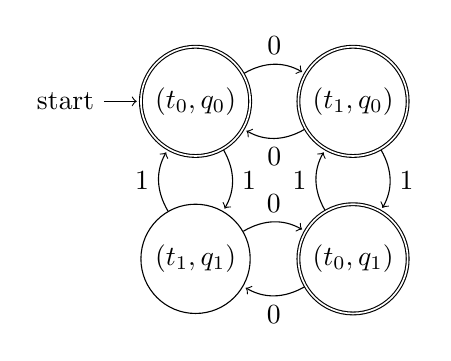
\begin{tikzpicture}[shorten >=1pt,node distance=2cm,on grid,auto]
     \node[state, initial, accepting] (t_0q_0)   {$(t_0, q_0)$};
     \node[state, accepting] (t_1q_0) [right=of t_0q_0] {$(t_1, q_0)$};
     \node[state, accepting] (t_0q_1) [below=of t_1q_0] {$(t_0, q_1)$};
     \node[state] (t_1q_1) [below=of t_0q_0] {$(t_1, q_1)$};
      \path[->]
      (t_0q_0) edge [bend left]  node {0} (t_1q_0)
               edge [bend left]  node {1} (t_1q_1)
      (t_1q_0) edge [bend left]  node {1} (t_0q_1)
               edge [bend left]  node {0} (t_0q_0)
      (t_0q_1) edge [bend left]  node {1} (t_1q_0)
               edge [bend left]  node {0} (t_1q_1)
      (t_1q_1) edge [bend left]  node {1} (t_0q_0)
               edge [bend left]  node {0} (t_0q_1);
    \end{tikzpicture}
  \end{center}
  Here we define predicate
  \[
    P(x): \delta^{*}((t_0, q_0), x) =
    \begin{cases}
      (t_0, q_0), & x \text{ has even number of characters and even number of 1's} \\
      (t_1, q_0), & x \text{ has odd number of characters and even number of 1's} \\
      (t_0, q_1), & x \text{ has even number of characters and odd number of 1's} \\
      `(t_1, q_1)`, & x \text{ has odd number of characters and odd number of 1's} \\
    \end{cases}
   \]
  Now we use structural induction to prove that $P(x)$ holds for all strings $x\in \Sigma^*$
  \begin{proof}
    $ $\\
    \textbf{Basis:}\\
    let $x=\epsilon$, $x$ in this case has zero of 0s and zero 1s. So $x$ is a string with even number of characters and even number of 1s and also $\delta^* ((t_0, q_0), x) = (t_0, q_0)$. Therefore $P(x)$ holds \\
    \textbf{Inductive step:} \\
    Let $x = ya$, where $y\in \Sigma^*$ and $a\in \Sigma$. Now assume $P(y)$ holds; this is the inductive hypothesis. We prove that $P(x)$ also holds. \\
    \textbf{Case 1:} when $a=0$\\
    \begin{align*}
      \delta^* &((t_0, q_0), x) \\
      &= \delta^* ((t_0, q_0), y0) \\
      &= \delta( \delta^*((t_0, q_0), y), 0) \\
      &= \begin{cases}
        \delta((t_0, q_0), 0), & y \text{ has even number of characters and even number of 1's} \\
        \delta((t_1, q_0), 0), & y \text{ has odd number of characters and even number of 1's} \\
        \delta((t_0, q_1), 0), & y \text{ has even number of characters and odd number of 1's} \\
        \delta((t_1, q_1), 0), & y \text{ has odd number of characters and odd number of 1's} \\
      \end{cases} \text{ by I.H. P(y) holds}\\
      & \text{because x has one more character and one more zero, we have}\\
      &= \begin{cases}
        (t_1, q_0), & x \text{ has odd number of characters and even number of 1's} \\
        (t_0, q_0), & x \text{ has even number of characters and even number of 1's} \\
        (t_1, q_1), & x \text{ has odd number of characters and odd number of 1's} \\
        (t_0, q_1), & x \text{ has even number of characters and odd number of 1's} \\
      \end{cases} \text{ by transition function}
    \end{align*}
    Therefore, $P(x)$ holds in this case.\\
    \textbf{Case 2:}\\
    Similar to Case 1 we arrive at $P(x)$ holds in this case. \\
    Therefore, $P(x)$ holds for all strings $x\in \Sigma^*$ by structural induction

    We proved that $P(x)$ is a state invariant for $M_3$


  \end{proof}

\end{solution}
\end{enumerate}

\section*{Problem 3}

Equivalence of languages and regular expressions \\
Language $L$ over alphabet $\Sigma=\{a,b\}$ consists of all strings that start with $a$ and have odd lengths or start with $b$ and have even lengths: $\{s | s$ starts with a and has odd length, or starts with b and has even length$\}$.
\begin{enumerate}
\item What is a regular expression $R$ corresponding to language $L$?
\[
  R = a((a+b)(a+b))^* + b(a+b)((a+b)(a+b))^*
\]
\item Prove that your regular expression $R$ is indeed equivalent to $L$

\begin{proof}
  $ $\\
  Here we denote $L(R)$ as the language described by $R$ over alpabet $\Sigma$. We show containment in both directions to prove equivalence, i.e.,
  \[
    L(R) = L \iff L(R)\subseteq L \land L\subseteq L(R)
  \]
  To prove $L(R)\subseteq L$, let $x\in L(R)$, then by definition of regular language,
  \[
    x\in L(a((a+b)(a+b))^*) \cup L(b(a+b)((a+b)(a+b))^*)
  \]
  \textbf{Case 1:} When $x\in L(a((a+b)(a+b))^*)$\\
  Then $x \in L(a)\circ (L((a+b)(a+b))^*$. Let $y\in L(a) = \{ a\}$, $w\in L((a+b)(a+b) = \{ aa, ab, ba, bb\}$. Then $y=a$ and $w^*$ is just concatenation of strings in $\{ aa, ab, ba, bb\}$, where the length of any string in the set is 2. Here $\exists k\in \N, | w^* | = 2k$ as follows. Therefore $yw^*$ is of length $2k+1$, hence odd. Note that $x=yw^*$, then $x$ is a string that starts with $a$ and has odd length. We see that $x\in L$ as expected.\\
  \textbf{Case 2:} When $x\in L(b(a+b)((a+b)(a+b))^*)$\\
  Then $x\in L(a)\circ L(a+b)\circ L((a+b)(a+b))$. Let $y\in L(a) = \{ b\}$, $u\in L(a+b) = \{ a, b\}$, and $w\in L((a+b)(a+b)) = \{ aa, ab, ba, bb\}$. Then $y=b$, $u$ is either $a$ or $b$ so of length 1, and $w^*$ has length $2k$ for some $k$ as explained previously. Then $|yuw| = 1+1+2k = 2(1+k)$, hence even. Note $x=yuw$, therefore $x$ is a string that starts with $b$ and has even length. We see that $x\in L$ as expected. \\
  Therefore, $x\in L(a((a+b)(a+b))^* + b(a+b)((a+b)(a+b))^*) \Rightarrow x\in L$, we proved that $L(R)\subseteq L$ \\

  To prove $L\subseteq L(R)$, let $x\in L$. Then
  \[
    x\in \{s: s \text{ starts with a and has odd length}\}\cup \{s|s \text{ starts with b and has even length} \}
  \]
  \textbf{Case 1:} $x$ is a string that starts with $a$ and has odd length $2k+1$ for some $k\in\N$. Then the substring excluding prefix $a$ has even length $2k$. Let
  \[
    x=yw_1w_2 \dots w_k
  \]
  where $y=a$ and $w_i \in \{aa, ab, ba, bb\}$ for $1\leq i\leq k$. This construction is valid because $|y|=1$ and $| w_1w_2\dots w_k | = 2k$ and therefore $|x| = 1 + 2k$ is as wanted. Also we see that $y\in L(a)$ and $w_i\in L((a+b)(a+b))$. Because $x$ contains arbitrary $k$ number of $w_i$, then $w_1w_2 \dots w_k \in L((a+b)(a+b))^* = L(((a+b)(a+b))^*)$ Then $x \in L(a)\circ L(((a+b)(a+b))^*) = L(a((a+b)(a+b))^*)$. Therefore, $x\in L(a((a+b)(a+b))^*) \cup L(b(a+b)((a+b)(a+b))^*)$ as wanted.\\
  \textbf{Case 2:} $x$ starts with $b$ and has even length, $2k+2$ for some $k\in\N$ (i.e. $x$ cannot be empty). Then the substring excluding prefix $b$ has odd length $2k+1$. let
  \[
    x=yuw_1w_2 \dots w_k
  \]
  where $y=a$, $u\in\{ a,b\}$, and $w_i\in \{ aa,ab,ba, bb\}$ for $1\leq i \leq k$. This construction is valid because $|y|=1$, $|u|=1$ and $|w_1w_2 \dots w_k| = 2k$ and therefore $|x| = 2+2k$ as wanted. Also note that $y\in L(a)$, $u\in L(a+b)$, $w_i \in L((a+b)(a+b))$. Because $x$ contains arbitrary number $k$ of $w_i$, then $w_1w_2 \dots w_k\in L((a+b)(a+b))^* = L(((a+b)(a+b))^*)$. Then by $x=yuw_1w_2 \dots w_k$, $x\in L(a)\circ L(a+b) \circ L(((a+b)(a+b))^*) = L(a(a+b)((a+b)(a+b))^*)$. Therefore $x\in L(a((a+b)(a+b))^*) \cup L(b(a+b)((a+b)(a+b))^*)$ as wanted. \\

  Since $x\in L \Rightarrow x\in L(R)$, we proved that $L\subseteq L(R)$.\\

  To conclude, because $L(R)\subseteq L \land L\subseteq L(R)$, then $L = L(R)$.

\end{proof}
\end{enumerate}


\end{document}
